\documentclass[12pt]{article}

\usepackage{amsmath, amssymb, amsthm, enumerate, graphicx}
\usepackage[usenames,dvipsnames]{color}
\usepackage{bm}
\usepackage[colorlinks=true,urlcolor=blue]{hyperref}
\usepackage{geometry}
\geometry{margin=1in}
\usepackage{float}
\usepackage{graphics}
\setlength{\marginparwidth}{2.15cm}
\usepackage{booktabs}
\usepackage{enumitem}
\usepackage{epsfig}
\usepackage{setspace}
\usepackage{parskip}
\usepackage[normalem]{ulem}
\usepackage{tikz}
\usetikzlibrary{positioning, arrows, automata}
\usepackage{pgfplots}
\usepackage[font=scriptsize]{subcaption}
\usepackage{float}
\usepackage[]{algorithm2e}
\usepackage{environ}
\usepackage{bbm}
\usepackage{graphicx}
\usepackage{titling}
\usepackage{url}
\usepackage{xcolor}
\usepackage{lipsum}
\usepackage{lastpage}
\usepackage[colorlinks=true,urlcolor=blue]{hyperref}
\usepackage{multicol}
\usepackage{tabularx}
\usepackage{comment}
\usepackage[utf8]{inputenc}
\usepackage{amssymb}
\usepackage{setspace}
\usepackage{marvosym}
\usepackage{wrapfig}
\usepackage{datetime}
\usepackage[many]{tcolorbox}
\usepackage{array}
\usepackage{multirow}
\usepackage{wasysym}
\usepackage{cancel}
\usepackage{xcolor} 
\usepackage{listings}
\usepackage{color}
\usepackage[thinlines]{easytable}
\usepackage{lastpage}

\newcommand{\R}{\mathbb{R}}
\newcommand{\blackcircle}{\tikz\draw[black,fill=black] (0,0) circle (1ex);}
\renewcommand{\circle}{\tikz\draw[black] (0,0) circle (1ex);}

\usetikzlibrary{positioning,calc}

\newtcolorbox[]{solution}[1][]{%
    breakable,
    enhanced,
    colback=white,
    %title=Solution,
    #1
}

\begin{document}
\section*{}
\begin{center}
  \centerline{\textsc{\LARGE  Homework 1 Template}}
\end{center}

Use this template to record your answers for Homework 1.  Add your answers using \LaTeX and then save your document as a PDF to upload to Gradescope.  You are required to use this template to submit your answers.  \textbf{You should not alter this template in any way} other than to insert your solutions.  You must submit all \pageref{LastPage} pages of this template to Gradescope.  Do not remove the instructions page(s).  Altering this template or including your solutions outside of the provided boxes can result in your assignment being graded incorrectly.  You may lose points if you do not follow these instructions.

Instructions to upload code have been provided in the handout.

\section*{Instructions for Specific Problem Types}

On this homework, you must fill in the blank for each problem; please make sure your final answer is fully included in the given space.  \textbf{Do not change the size of the box provided.}  For short answer questions you should \textbf{not} include your work in your solution.  Only provide an explanation or proof if specifically asked.  Otherwise, your assignment may not be graded correctly, and points may be deducted from your assignment.

\begin{quote}
\textbf{Fill in the blank:} What is the course number?

\begin{tcolorbox}[fit,height=1cm, width=4cm, blank, borderline={1pt}{-2pt},valign=center,nobeforeafter]
    \begin{center}\huge10-703\end{center}
    \end{tcolorbox}
\end{quote}

\newpage

\section*{Problem 0: Collaborators}
Enter your team's names and Andrew IDs in the boxes below.  If you do not do this, you may lose points on your assignment.

Name 1: \begin{tcolorbox}[fit,height=1cm, width=5cm, blank, borderline={1pt}{1pt},nobeforeafter]
    \begin{center}
    \vspace{3mm}
    \large{Mike Anoruo}
    \end{center}
\end{tcolorbox}
Andrew ID 1: \begin{tcolorbox}[fit,height=1cm, width=5cm, blank, borderline={1pt}{1pt},nobeforeafter]
    \begin{center}
    \vspace{3mm}
    \large{manoruo}
    \large{}
    \end{center}
\end{tcolorbox}
    \\
Name 2: \begin{tcolorbox}[fit,height=1cm, width=5cm, blank, borderline={1pt}{1pt},nobeforeafter]
    \begin{center}
    \vspace{3mm}
    \large{}
    \end{center}
\end{tcolorbox}
Andrew ID 2: \begin{tcolorbox}[fit,height=1cm, width=5cm, blank, borderline={1pt}{1pt},nobeforeafter]
    \begin{center}
    \vspace{3mm}
    \large{}
    \end{center}
\end{tcolorbox} \\
Name 3: \begin{tcolorbox}[fit,height=1cm, width=5cm, blank, borderline={1pt}{1pt},nobeforeafter]
    \begin{center}
    \vspace{3mm}
    \large{}
    \end{center}
\end{tcolorbox}
Andrew ID 3: \begin{tcolorbox}[fit,height=1cm, width=5cm, blank, borderline={1pt}{1pt},nobeforeafter]
    \begin{center}
    \vspace{3mm}
    \large{}
    \end{center}
\end{tcolorbox} \\
\vspace{0.5cm}
\vspace{0.5cm}


\newpage
\section*{Problem 1: REINFORCE (48 pts)}

\subsection*{1.1 Reinforce plot (10 pts)}
\begin{solution}[height=9cm]
% YOUR SOLUTION
\begin{center}
    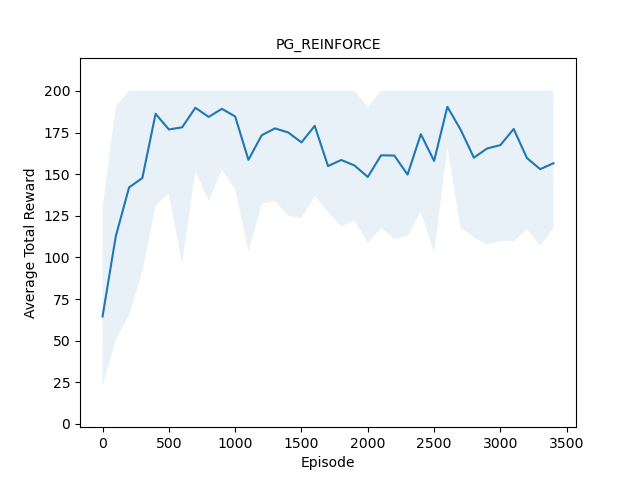
\includegraphics[width=0.7\textwidth,keepaspectratio]{code/pg/graphs/PG_REINFORCE.png}
\end{center}
\end{solution}

\subsection*{1.2 Reinforce with baseline plot (10 pts)}
\begin{solution}[height=9cm]
% TODO: Put your figures
\begin{center}
    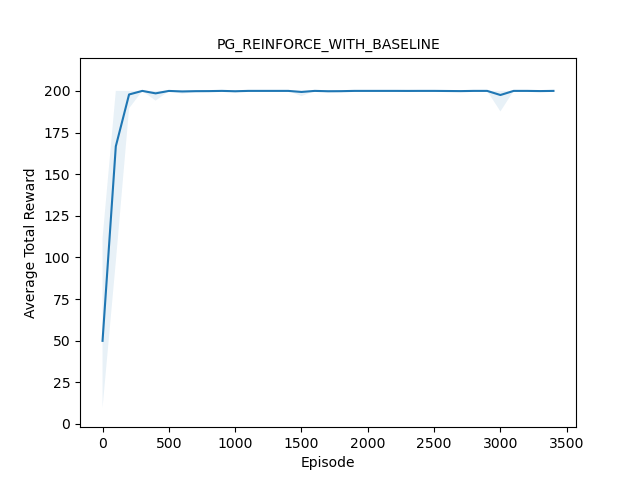
\includegraphics[width=0.7\textwidth,keepaspectratio]{code/pg/graphs/PG_REINFORCE_WITH_BASELINE.png}
\end{center}
% YOUR SOLUTION
\end{solution}

\subsection*{1.3 N-step A2C (20 pts)}
\begin{solution}[height=20cm]
% TODO: Put your figures
\begin{center}
    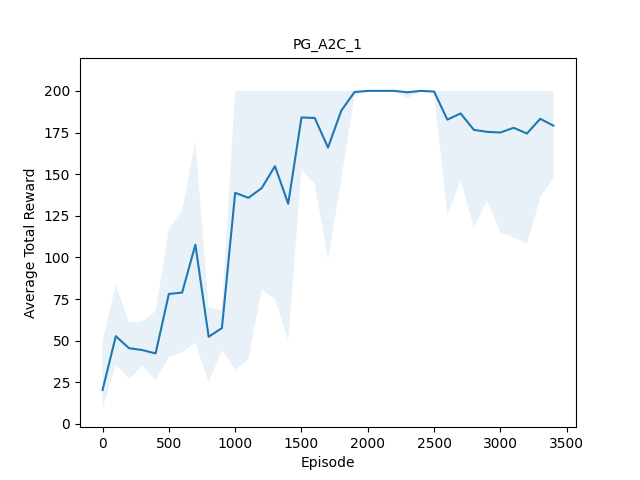
\includegraphics[width=0.5\textwidth,keepaspectratio]{code/pg/graphs/PG_A2C_1.png}
    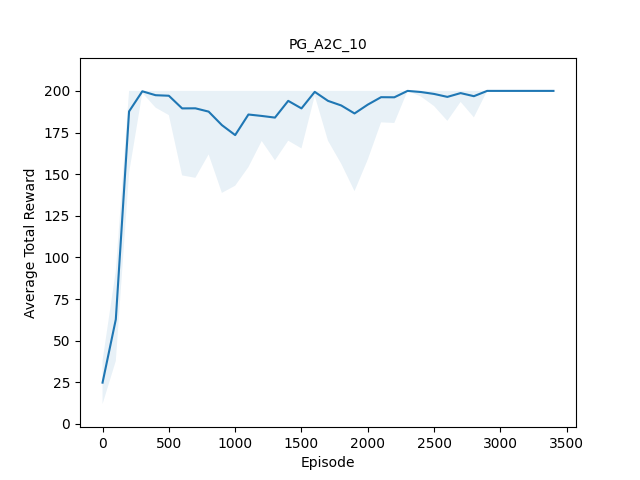
\includegraphics[width=0.5\textwidth,keepaspectratio]{code/pg/graphs/PG_A2C_10.png}
    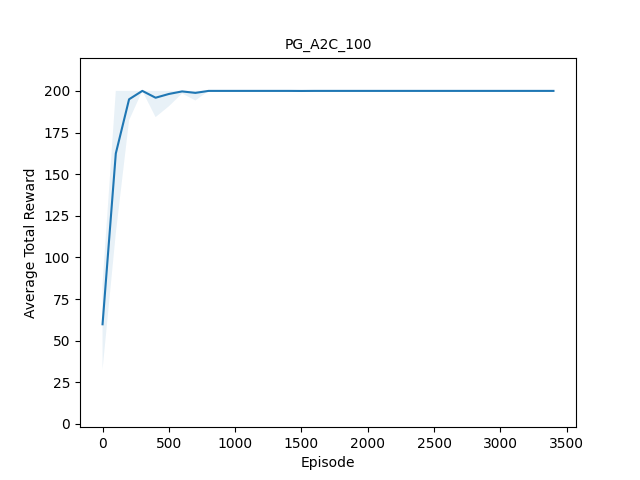
\includegraphics[width=0.5\textwidth,keepaspectratio]{code/pg/graphs/PG_A2C_100.png}
\end{center}
% YOUR SOLUTION
\end{solution}

\subsection*{1.4 N-step A2C \& REINFORCE with baseline (4 pts)}
\begin{solution}[height=5cm]
% TODO: Put your figures
% YOUR SOLUTION
N-step A2C, REINFORCE, and REINFORCE with baseline are all policy gradient methods that update the policy to increase the probability of actions leading to higher returns. 
\begin{itemize}
    \item \textbf{N-step A2C $\rightarrow$ REINFORCE with baseline:} when $n=T$, i.e., the return is computed over the entire episode (full-horizon), so no bootstrapping is used.
    \item \textbf{N-step A2C or REINFORCE with baseline $\rightarrow$ REINFORCE:} if the baseline $V(s_t)$ is zero (or not used), then both reduce to plain REINFORCE.
\end{itemize}

\end{solution}

\subsection*{1.5 REINFORCE with \& without baseline (4 pts)}
\begin{solution}[height=5cm]
% TODO: Put your figures
% YOUR SOLUTION
Adding a baseline generally improves performance by reducing the variance of the policy gradient estimates, 
which allows the model to converge faster. 
The baseline acts like a "standard" or reference point for expected return from a state. 
Actions that lead to rewards higher than this standard are reinforced, 
while actions that fall below it are not. 
Without a baseline, REINFORCE tends to reinforce all actions in a trajectory that eventually lead to a reward, 
even if some of them didn't necessarily contribute to it. 
By using a baseline, the algorithm puts more "blame" or "credit" on actions that truly affect the outcome, 
reducing noise and improving learning efficiency.

\end{solution}

\section*{2 Question Answering (12 pts)}
\begin{enumerate}
    \item \noindent\begin{solution}[height=5cm] 
    \end{solution}

    \item \noindent\begin{solution}[height=5cm]
        False. Q-learning requires exploration during training to discover optimal actions in all states. If it only follows the greedy policy over the current Q function, it may get stuck in suboptimal trajectories and fail to maximize long-term rewards.
    \end{solution}

    \item \noindent\begin{solution}[height=5cm]
    False. By definition, $v^{\pi^*}(s)$ is the value under the optimal policy, which is always at least as large as the value under any other policy. No policy can have a higher value at a state than the optimal policy.
    \end{solution}

    \item \noindent\begin{solution}[height=5cm]
    False. Actor-critic methods can optimize policies over discrete actions using a parameterized policy, such as a softmax output to represent action probabilities.
    \end{solution}

    \item \noindent\begin{solution}[height=5cm]
    False. Actor-critic methods typically use stochastic policies (e.g., softmax) to explore, rather than epsilon-greedy, which is primarily used in Q-learning.
    \end{solution}

    \item \noindent\begin{solution}[height=5cm]
    \begin{itemize}
        \item Switching to $a_1$ for state $s$ will provide us with a policy better than $\pi$. \textbf{(Only correct answer)}
    \end{itemize}
    Changing the action at state $s$ to the higher-Q action $a_1$ improves the policy at that state. We cannot guarantee that other states’ values will decrease, nor that the resulting policy is globally optimal if other states are still suboptimal.
    \end{solution}

    \item \noindent\begin{solution}[height=5cm]
    \end{solution}
\end{enumerate}




\clearpage
\section*{Feedback}

\textbf{Feedback}: You can help the course staff improve the course for future semesters by providing feedback. You will receive a point of you provide actionable feedback. What was the most confusing part of this homework, and what would have made it less confusing?
\begin{solution}[height=4cm]
    I had some confusion with the difference between A2C and REINFORCE with baseline. From the lecture, it seemed like this REINFORCE with baseline was the same as actor critic since we werent subtracting a constant value. I wasnt sure though since the homework didnt call it this. Also some template code for the size of the graphics would be good. Wasn't sure how big to make the images without making them too small or too big.
\end{solution}

\textbf{Collaboration}: Detail the work division amongst your group below.
\begin{solution}[height=4cm]
    Worked on this assignment individually.
\end{solution}

\noindent\textbf{Time Spent}: How many hours did you spend working on this assignment? Your answer will not affect your grade. Please average your answer over all the members of your team.
\begin{solution}[height=4cm]
\begin{table}[H]
    \centering
    \begin{tabular}{r|c}
        Alone &  \hspace{3em} 16 %ANSWER HERE%
        \\ \hline
        With teammates & \hspace{3em} 0  %ANSWER HERE%
        \\ \hline
        With other classmates & \hspace{3em} 0 %ANSWER HERE%
        \\ \hline
        At office hours & \hspace{3em} 0 %ANSWER HERE%
        \\ \hline
    \end{tabular}
\end{table}
\end{solution}


\end{document}
